% Informe – Primera entrega
% Sistema distribuido de transacciones para eventos universitarios
%
% Compilar en Overleaf con pdfLaTeX (Menu → Compiler → pdfLaTeX).
\documentclass[11pt,letterpaper]{article}

% ------------------------------------------------------------------ Idioma y fuentes
\usepackage[utf8]{inputenc}
\usepackage[T1]{fontenc}
\usepackage[spanish,es-noshorthands,es-tabla]{babel}
\usepackage{lmodern}
\usepackage{microtype}

% ------------------------------------------------------------------ Página
\usepackage[margin=2.3cm]{geometry}
\usepackage{fancyhdr}
\usepackage{titlesec}
\usepackage{enumitem}
\setlist{nosep, leftmargin=*}
\setlength{\parskip}{0.45em}
\setlength{\parindent}{0pt}

% ------------------------------------------------------------------ Tablas, figuras y código
\usepackage{graphicx}
\usepackage{float}
\usepackage{rotating}
\usepackage{caption}
\captionsetup{font=small, labelfont=bf}
\usepackage{booktabs}
\usepackage{tabularx}
\usepackage{longtable}
\usepackage{multirow}
\usepackage{array}
\newcolumntype{Y}{>{\raggedright\arraybackslash}X}
\renewcommand{\arraystretch}{1.18}
\usepackage{xcolor}
\usepackage{listings}
\usepackage{amsmath}

% ------------------------------------------------------------------ Diagramas
\usepackage{tikz}
\usetikzlibrary{babel, positioning, arrows.meta, shapes.geometric, shapes.multipart,
                fit, backgrounds, calc, shadows}
\usepackage{pgf-umlsd}
\usepackage{pgf-umlcd}
\usepackage{pgfplots}
\pgfplotsset{compat=1.18}

\usepackage[hidelinks]{hyperref}

% ------------------------------------------------------------------ Estilo
\definecolor{azul}{RGB}{31,78,121}
\definecolor{azulclaro}{RGB}{222,235,247}
\definecolor{naranja}{RGB}{237,125,49}
\definecolor{verde}{RGB}{146,208,80}
\definecolor{morado}{RGB}{112,48,160}
\definecolor{gris}{RGB}{110,110,110}

\titleformat{\section}{\Large\bfseries\color{azul}}{\thesection}{0.6em}{}
\titleformat{\subsection}{\large\bfseries\color{azul}}{\thesubsection}{0.6em}{}
\titleformat{\subsubsection}{\normalsize\bfseries}{\thesubsubsection}{0.6em}{}

\lstset{basicstyle=\ttfamily\small, columns=fullflexible, keepspaces=true,
        frame=single, rulecolor=\color{gris!50}, backgroundcolor=\color{gris!6},
        breaklines=true, showstringspaces=false,
        literate={á}{{\'a}}1 {é}{{\'e}}1 {í}{{\'i}}1 {ó}{{\'o}}1 {ú}{{\'u}}1 {ñ}{{\~n}}1}

\pagestyle{fancy}
\fancyhf{}
\lhead{\small Sistemas Distribuidos – Primera entrega}
\rhead{\small Eventos universitarios}
\cfoot{\thepage}

\newcommand{\codigo}[1]{\texttt{#1}}

% ------------------------------------------------------------------ Datos de la portada (completar)
\newcommand{\universidad}{Nombre de la universidad}
\newcommand{\curso}{Sistemas Distribuidos}
\newcommand{\profesor}{Nombre del profesor}
\newcommand{\repositorio}{\url{https://github.com/x19marlon/proyecto_distribuidos}}

\begin{document}

% ------------------------------------------------------------------ Portada
\begin{titlepage}
    \centering
    {\large \universidad\par}
    \vspace{0.3cm}
    {\large \curso\par}
    \vspace{3cm}
    {\color{azul}\rule{\linewidth}{1.2pt}\par}
    \vspace{0.4cm}
    {\Huge\bfseries Sistema distribuido de transacciones\\[0.2cm] para eventos universitarios\par}
    \vspace{0.4cm}
    {\Large Primera entrega: modelos, diseño y plan de pruebas\par}
    \vspace{0.2cm}
    {\color{azul}\rule{\linewidth}{1.2pt}\par}
    \vspace{2.5cm}
    {\large Equipo \textbf{crotolamo que gico}\par}
    \vspace{0.6cm}
    \begin{tabular}{c}
        mariananvv16 \\
        martinezm-oe \\
        Nick\_07 \\
        x19marlon
    \end{tabular}
    \vfill
    {\large Profesor: \profesor\par}
    \vspace{0.3cm}
    {\large \today\par}
    \vspace{0.3cm}
    {\small Repositorio: \repositorio\par}
\end{titlepage}

\tableofcontents
\newpage

\section{Introducción}

\subsection{Contexto}

La universidad organiza cada semestre una gran cantidad de eventos abiertos a sus
estudiantes: conciertos, talleres, conferencias, ferias y actividades culturales.
Algunos se realizan en edificios o teatros del campus, cuya capacidad es conocida,
y otros en lugares externos. Un mismo evento puede repetirse en varias fechas, y
algunos son gratuitos mientras que otros tienen un costo por cupo.

Hoy la inscripción a estos eventos suele hacerse con formularios independientes,
hojas de cálculo o directamente en la entrada del evento. Esto hace difícil saber
cuántos cupos quedan, permite que se inscriban más personas que la capacidad del
lugar y no deja un registro confiable de quién reservó, modificó o canceló.

En el curso de Sistemas Distribuidos se propone construir un \textbf{sistema
distribuido de transacciones} que resuelva este problema y que, al mismo tiempo,
permita estudiar en la práctica los conceptos del curso: arquitecturas por capas,
comunicación por paso de mensajes, modelos de interacción, de fallos y de
seguridad, tolerancia a fallos, escalabilidad y evaluación de desempeño.

\subsection{Problema}

Se necesita un sistema al que muchos estudiantes accedan al mismo tiempo desde
distintas máquinas para:

\begin{itemize}
    \item consultar los eventos programados en un mes y los cupos disponibles de cada fecha;
    \item reservar uno o más cupos en una fecha de un evento;
    \item modificar una reserva (cantidad de cupos o fecha), y
    \item cancelar una reserva.
\end{itemize}

Las consultas, reservas y modificaciones deben responder de forma \textbf{síncrona}:
el estudiante espera y recibe el resultado definitivo en la misma operación. La
cancelación es \textbf{asíncrona}: el sistema la acepta de inmediato, informa que
está en proceso y la aplica después en la capa de datos.

El problema es distribuido por naturaleza: los clientes, los servicios de negocio y
el almacenamiento corren en procesos y máquinas distintas que se comunican por la
red. Esto introduce dificultades que no existen en un programa centralizado:
\begin{itemize}
    \item \textbf{Concurrencia:} dos estudiantes pueden pedir el último cupo al mismo
          tiempo y el sistema nunca debe superar la capacidad de una fecha.
    \item \textbf{Fallos parciales:} un proceso puede caerse o un mensaje perderse; un
          reintento no debe reservar ni cobrar dos veces, y una cancelación aceptada no
          debe perderse.
    \item \textbf{Desempeño:} cada transacción debe completarse en menos de un segundo,
          y el desempeño debe medirse y compararse entre una arquitectura base y una
          escalable (Tabla~1 del enunciado).
    \item \textbf{Seguridad:} se manejan datos personales de los estudiantes y dinero.
\end{itemize}

\subsection{Objetivos}

\paragraph{Objetivo general.} Diseñar, implementar y evaluar un sistema distribuido
de tres capas (consumidores, servicios de negocio y almacenamiento), comunicado con
ZeroMQ, que gestione las reservas de eventos universitarios de forma consistente,
tolerante a fallos y con tiempos de respuesta menores a un segundo.

\paragraph{Objetivos específicos.}
\begin{enumerate}
    \item Describir el sistema con los modelos arquitectónico, de interacción, de
          fallos y de seguridad, y mostrar cómo cada uno condiciona el diseño.
    \item Diseñar la arquitectura base de la Figura~\ref{fig:arquitectura-basica} con
          diagramas UML de despliegue, componentes, clases y secuencia.
    \item Implementar en C++ orientado a objetos los componentes de la arquitectura
          base con las operaciones de consulta y reserva.
    \item Identificar y justificar los componentes que harán la arquitectura escalable
          y tolerante a fallos en la segunda entrega.
    \item Definir el protocolo de pruebas del sistema, las herramientas para obtener
          las métricas de desempeño de la Tabla~1 y el método de generación de carga.
\end{enumerate}

\subsection{Alcance de esta entrega}

Este documento corresponde a la \textbf{primera entrega}. Contiene los modelos del
sistema, el diseño completo de la arquitectura base (incluidas la modificación y
la cancelación asíncrona), la justificación de los componentes de escalabilidad y
tolerancia a fallos, el protocolo de pruebas y la estrategia de medición. La
implementación entregada cubre las operaciones de \textbf{consulta y reserva}
sobre los componentes de la arquitectura base (sección~\ref{sec:implementacion}).

\section{Modelos del sistema}
\label{sec:modelos}

Siguiendo a Coulouris et al.~\cite{coulouris}, el sistema se describe con cuatro
modelos. Para cada uno se presentan los conceptos y cómo se aplican al proyecto.

% =====================================================================
\subsection{Modelo arquitectónico}

El modelo arquitectónico define qué entidades forman el sistema, cómo se comunican,
qué papel cumple cada una y dónde se ubican.

\subsubsection{Estilo arquitectónico}

\begin{table}[H]
\centering
\caption{Estilos arquitectónicos aplicados al proyecto.}
\begin{tabularx}{\textwidth}{>{\bfseries}p{3.6cm}Y}
\toprule
Concepto & Cómo se aplica \\
\midrule
Arquitectura por capas &
Tres capas en orden estricto: \emph{Consumidores} $\rightarrow$ \emph{Servicios de
Negocio} $\rightarrow$ \emph{Servicios de Almacenamiento}. Cada capa solo llama a la
capa inmediatamente inferior, por lo que cada una puede desplegarse, reemplazarse y
escalarse por separado. \\
Cliente--servidor &
Los clientes son clientes del \codigo{GestorTransacciones}; a su vez, los procesos
de negocio son clientes del Servicio de Persistencia. \\
Intermediario (broker) &
El \codigo{GestorTransacciones} es el único punto de entrada: los clientes solo
conocen su dirección y él reparte las peticiones entre los procesos de negocio. Los
clientes quedan desacoplados de cuántos procesadores hay y dónde están. \\
Servicios sin estado &
Gestor, procesadores y servicio de cancelación no guardan datos de negocio en
memoria; todo el estado vive en la capa de almacenamiento. Por eso pueden
reiniciarse o replicarse sin perder información. \\
Publicación--suscripción &
Las cancelaciones se anuncian con ZeroMQ \codigo{PUB}/\codigo{SUB}: el gestor
publica sin conocer a los suscriptores (desacoplamiento en el espacio) y la
solicitud guardada permite aplicarla después (desacoplamiento en el tiempo). \\
Fuente única de verdad &
El Servicio de Persistencia es el único que decide los cupos, las reservas y las
transacciones, lo que simplifica la consistencia. \\
\bottomrule
\end{tabularx}
\end{table}

\subsubsection{Entidades y roles}

Las entidades corresponden a las cajas de la Figura~\ref{fig:arquitectura-basica}.
Cada una es un proceso independiente:

\begin{table}[H]
\centering
\caption{Procesos del sistema.}
\begin{tabularx}{\textwidth}{p{4.1cm}p{2.6cm}Y}
\toprule
Proceso & Capa & Responsabilidad \\
\midrule
\codigo{cliente} & Consumidores & Interfaz del estudiante: consultar eventos del mes,
reservar, modificar y cancelar; recibe notificaciones de cancelación. \\
\codigo{gestor-transacciones} & Servicios de Negocio & Recibe todas las solicitudes,
envía las síncronas a un procesador RMC libre y publica las cancelaciones. \\
\codigo{procesador-rmc} & Servicios de Negocio & Procesamiento de
\textbf{R}eservas, \textbf{M}odificaciones y \textbf{C}onsultas: valida y ejecuta
las operaciones síncronas contra persistencia. \\
\codigo{cancelacion-reservas} & Servicios de Negocio & Aplica de forma asíncrona las
cancelaciones aceptadas y notifica el resultado al estudiante. \\
\codigo{persistencia} & Servicios de Almacenamiento & Guarda estudiantes, lugares,
eventos, fechas, reservas y transacciones; aplica cada cambio de forma atómica. \\
\bottomrule
\end{tabularx}
\end{table}

\subsubsection{Paradigmas de comunicación}

Toda la comunicación entre procesos usa paso de mensajes con ZeroMQ~\cite{zguide}:

\begin{itemize}
    \item \textbf{Petición--respuesta} (\codigo{REQ}/\codigo{ROUTER}/\codigo{DEALER}/\codigo{REP})
          para consultas, reservas y modificaciones, y para la aceptación de la
          cancelación. Quien llama se bloquea hasta recibir la respuesta.
    \item \textbf{Publicación--suscripción} (\codigo{PUB}/\codigo{SUB}) para anunciar
          una cancelación aceptada al servicio de cancelación y para notificar el
          resultado al estudiante. El publicador no espera.
\end{itemize}

\subsubsection{Ubicación física}

En la arquitectura base cada proceso corre en una máquina del laboratorio
(sección~\ref{sec:despliegue}): una máquina para los clientes, una para el
gestor, una para los procesos de negocio y una para persistencia. Las direcciones y
puertos se leen de variables de entorno, de modo que el mismo programa corre en una
sola máquina (desarrollo) o repartido en varias (pruebas). En la segunda entrega el
sistema se desplegará en Kubernetes sobre las mismas 4 máquinas
(sección~\ref{sec:escalabilidad}).

% =====================================================================
\subsection{Modelo de interacción}

El modelo de interacción trata el desempeño de los canales, la ausencia de un reloj
global y el orden de los eventos.

\subsubsection{Sistema asíncrono y cotas prácticas}

En un \emph{sistema distribuido síncrono} existen cotas conocidas para el tiempo de
ejecución de los procesos, el retardo de los mensajes y la deriva de los relojes;
en uno \emph{asíncrono} no existen. La red del laboratorio no garantiza ninguna
cota, así que el sistema corre sobre un modelo \textbf{asíncrono}. Que las
operaciones sean ``síncronas'' se refiere al \emph{estilo de interacción} (el
cliente espera la respuesta), no a tiempos garantizados.

Para poder actuar, el sistema asume \textbf{cotas prácticas} mediante timeouts:
\begin{itemize}
    \item cliente $\rightarrow$ gestor: 1\,s por intento, hasta 3 intentos;
    \item procesos de negocio $\rightarrow$ persistencia: 300\,ms por intento, hasta 3 intentos;
    \item latidos (\emph{heartbeats}) entre gestor y procesadores cada 1\,s; tres
          perdidos significan que el procesador está caído.
\end{itemize}
Cuando se vence un timeout el resultado se considera \textbf{desconocido}, no
fallido: la operación pudo haberse aplicado. Por eso los reintentos deben ser
idempotentes (sección~\ref{sec:semantica}).

\subsubsection{Desempeño de los canales}

\begin{itemize}
    \item \textbf{Latencia:} ZeroMQ mantiene conexiones TCP persistentes entre
          procesos, así que no se paga un establecimiento de conexión por petición.
    \item \textbf{Ancho de banda:} los mensajes son pequeños (texto
          \codigo{clave=valor}); la consulta de un mes devuelve pocas decenas de filas.
    \item \textbf{Jitter:} se observa comparando el promedio con la desviación
          estándar y el percentil 95 en las pruebas de la Tabla~1.
\end{itemize}

\subsubsection{Relojes y orden de los eventos}

Cada máquina tiene su propio reloj y estos derivan. Por eso:
\begin{itemize}
    \item Las \textbf{duraciones} (tiempos de respuesta) se miden siempre con el reloj
          monótono de una sola máquina: inicio y fin en el mismo proceso cliente.
    \item El \textbf{orden de las operaciones} sobre los mismos datos lo decide el
          Servicio de Persistencia, que atiende las peticiones una a una. Si dos
          estudiantes compiten por el último cupo, gana el que persistencia procesa
          primero, no el que tenga la marca de tiempo menor.
    \item Las marcas de tiempo guardadas (instante de una transacción) las pone
          siempre persistencia, así que son consistentes entre sí.
    \item Cada operación lleva un \codigo{idSolicitud} único que permite seguirla a
          través de los procesos en los registros.
\end{itemize}

\subsubsection{Semántica de invocación}
\label{sec:semantica}

\begin{table}[H]
\centering
\caption{Semántica de invocación por operación.}
\begin{tabularx}{\textwidth}{p{4.2cm}p{2.6cm}Y}
\toprule
Operación & Estilo & Semántica \\
\midrule
Consultar eventos del mes & Síncrona & \emph{Al menos una vez}: los reintentos son
inofensivos porque es de solo lectura. \\
Reservar, modificar & Síncrona & \emph{Efectivamente exactamente una vez}: el
cliente reintenta con el mismo \codigo{idSolicitud} y persistencia devuelve la
respuesta guardada sin aplicar el cambio otra vez. \\
Cancelar (aceptación) & Síncrona, corta & Exactamente una solicitud de cancelación
guardada por \codigo{idSolicitud}. \\
Cancelar (aplicación) & Asíncrona & Entrega \emph{al menos una vez} (aviso
PUB/SUB + barrido periódico) y aplicación idempotente: la cancelación se aplica una
sola vez. \\
\bottomrule
\end{tabularx}
\end{table}

% =====================================================================
\subsection{Modelo de fallos}

El modelo de fallos define qué puede fallar, cómo falla y cómo el sistema lo detecta
y lo enmascara.

\subsubsection{Clases de fallos considerados}

\begin{table}[H]
\centering
\caption{Clases de fallos.}
\begin{tabularx}{\textwidth}{p{3.3cm}Y Y}
\toprule
Clase & Definición & Ejemplo en el proyecto \\
\midrule
Caída (\emph{fail-stop}) & El proceso se detiene y no hace nada más. &
Se apaga la máquina del procesador RMC. \\
Omisión de proceso & No envía o no recibe un mensaje. & El servicio de cancelación
se cae justo después de recibir un aviso. \\
Omisión de canal & El mensaje se pierde en la red. & Se pierde la respuesta de
\codigo{reservar}; el cliente agota el timeout. \\
Temporización & La respuesta llega, pero tarde. & Persistencia tarda más de 1\,s
bajo carga. \\
Arbitrario (bizantino) & Comportamiento incorrecto o malicioso. & Mensaje alterado
o cliente que envía datos inválidos. Queda fuera del modelo de corrección y lo
cubre en parte el modelo de seguridad. \\
\bottomrule
\end{tabularx}
\end{table}

\textbf{Supuestos.} (1) Los procesos fallan por caída. (2) Los canales pueden
perder, retrasar o duplicar mensajes, pero TCP detecta la corrupción. (3) Lo que
persistencia confirma como guardado sobrevive a una caída; los mensajes de ZeroMQ,
incluidos los de PUB/SUB, no son durables. (4) Desde afuera no se distingue una
caída de un proceso lento: un timeout solo significa ``desconocido''.

\subsubsection{Fallos por componente y cómo se enmascaran}

\begin{longtable}{p{3.1cm}p{3.6cm}p{8.6cm}}
\caption{Fallos por componente.}\\
\toprule
Componente & Fallo & Detección y manejo \\
\midrule
\endfirsthead
\toprule
Componente & Fallo & Detección y manejo \\
\midrule
\endhead
Red cliente--gestor & Se pierde la petición o la respuesta & Timeout del cliente;
reintento con el mismo \codigo{idSolicitud} (patrón \emph{Lazy Pirate}); no hay
reservas duplicadas. \\
Procesador RMC & Se cae con una petición en curso & El gestor deja de recibir sus
latidos y lo descarta; el cliente reintenta y otro procesador atiende. \\
Gestor de Transacciones & Se cae & Punto único de fallo en la arquitectura base; los
clientes reintentan hasta que se reinicie. Al volver, los procesadores se
registran de nuevo con su siguiente latido. En la segunda entrega se replica
(\emph{Binary Star}). \\
Servicio de cancelación & Se cae o pierde un aviso PUB/SUB & La solicitud ya quedó
guardada como \codigo{PENDIENTE}; un barrido periódico la encuentra y la aplica. \\
Persistencia & Se cae a mitad de una operación & Cada cambio es atómico (todo o
nada) y se escribe en disco antes de responder; al reiniciar se reconstruye el
estado. Los servicios responden \codigo{PERSISTENCIA\_NO\_DISPONIBLE}. \\
Persistencia & Lenta & Los indicadores de latencia lo muestran (p95 > 1\,s). \\
Relojes & Deriva entre máquinas & Las duraciones se miden en una sola máquina y el
orden lo decide persistencia. \\
\bottomrule
\end{longtable}

\subsubsection{Puntos únicos de fallo de la arquitectura base}

En la arquitectura base hay una sola instancia de cada componente, así que el
gestor, el servicio de cancelación y persistencia son puntos únicos de fallo. La
sección~\ref{sec:escalabilidad} presenta los componentes que los eliminan.

% =====================================================================
\subsection{Modelo de seguridad}

El modelo de seguridad identifica qué se protege, de quién y con qué defensas. Se
asume un \emph{enemigo} capaz de enviar cualquier mensaje a cualquier proceso y de
leer, copiar, alterar o repetir los mensajes que viajan por la red.

\subsubsection{Objetos a proteger}

\begin{itemize}
    \item \textbf{Datos personales del estudiante}: nombre, tipo y número de
          documento, correo, teléfono, carrera, departamento y semestre. En Colombia
          están protegidos por la Ley 1581 de 2012~\cite{ley1581}.
    \item \textbf{Reservas y cupos}: recurso limitado que podría acapararse.
    \item \textbf{Transacciones}: registro de auditoría de reservas, modificaciones y
          cancelaciones, con sus montos.
    \item \textbf{Eventos y lugares}: datos falsos engañarían a todos los estudiantes.
\end{itemize}

\subsubsection{Amenazas y defensas}

\begin{longtable}{p{3.0cm}p{5.0cm}p{7.3cm}}
\caption{Amenazas y defensas.}\\
\toprule
Amenaza & Ejemplo & Defensa \\
\midrule
\endfirsthead
\toprule
Amenaza & Ejemplo & Defensa \\
\midrule
\endhead
Suplantación & Cancelar la reserva de otro estudiante. & Autenticación del
estudiante (token de sesión) y verificación de propiedad: el
\codigo{idEstudiante} sale del token, nunca del cuerpo del mensaje
(\codigo{RESERVA\_AJENA}). Procesos internos autenticados con llaves CurveZMQ. \\
Escucha & Leer números de documento en la red. & Cifrado de todos los sockets con
CurveZMQ. \\
Alteración & Cambiar \codigo{cupos=1} por \codigo{cupos=50}. & CurveZMQ (cifrado
autenticado) y validación de rangos en el procesador RMC. \\
Repetición & Reenviar una reserva capturada. & \codigo{idSolicitud} único: la
repetición devuelve la respuesta guardada sin un segundo efecto. \\
Denegación de servicio & Inundar \codigo{reservar}. & Límite de solicitudes por
estudiante, colas acotadas de ZeroMQ (\emph{high-water marks}). \\
Elevación de privilegios & Un estudiante crea o borra eventos. & Autorización por
rol en la capa de negocio. \\
Fuga de datos & Documentos en los registros. & Los registros solo llevan
\codigo{idSolicitud} e \codigo{idEstudiante}; el documento se muestra enmascarado. \\
Repudio & ``Yo nunca cancelé''. & Toda operación queda como \codigo{Transaccion}
inmutable con estudiante, solicitud e instante. \\
Aislamiento & Conectarse directo a persistencia. & Solo el gestor es accesible desde
fuera; persistencia solo acepta conexiones de los procesos de negocio
(firewall o \emph{NetworkPolicy} en Kubernetes). \\
\bottomrule
\end{longtable}

\subsubsection{Seguridad frente a desempeño}

El cifrado agrega costo a cada mensaje. Como ZeroMQ mantiene conexiones
persistentes, el intercambio de llaves de CurveZMQ ocurre una sola vez por conexión
y no en cada petición. El costo se medirá comparando corridas con y sin cifrado.
En la primera entrega la autenticación y el cifrado no están implementados; se
incorporarán con los componentes de la sección~\ref{sec:escalabilidad}.

\section{Diseño del sistema: arquitectura base}
\label{sec:diseno}

% Diagramas de secuencia UML – arquitectura base
% Cada uno se define como un comando para incluirlo en su propia figura.
% Nota: en pgf-umlsd las etiquetas con paréntesis de \mess van entre llaves dobles.

\newcommand{\secuenciaConsultar}{%
{\footnotesize
\begin{sequencediagram}
    \newthread[morado!15]{c}{:Cliente}
    \newinst[1.6]{g}{:GestorTransacciones}
    \newinst[1.6]{r}{:ProcesadorRMC}
    \newinst[1.6]{p}{:ServicioPersistencia}
    \begin{call}{c}{consultarEventosMes(mes)}{g}{OK + filas}
        \begin{call}{g}{petición}{r}{respuesta}
            \begin{callself}{r}{validar AAAA-MM}{}
            \end{callself}
            \begin{call}{r}{listarFechasMes(mes)}{p}{OK + filas}
                \begin{callself}{p}{fechas del mes}{}
                \end{callself}
            \end{call}
        \end{call}
    \end{call}
\end{sequencediagram}}}

\newcommand{\secuenciaReservar}{%
{\footnotesize
\begin{sequencediagram}
    \newthread[morado!15]{c}{:Cliente}
    \newinst[1.6]{g}{:GestorTransacciones}
    \newinst[1.6]{r}{:ProcesadorRMC}
    \newinst[1.6]{p}{:ServicioPersistencia}
    \begin{call}{c}{reservar(idFecha, cupos)}{g}{OK idReserva}
        \begin{call}{g}{petición}{r}{respuesta}
            \begin{callself}{r}{validar datos}{}
            \end{callself}
            \begin{call}{r}{crearReserva}{p}{OK / ERROR}
                \begin{sdblock}{alt}{[idSolicitud ya procesado]}
                    \begin{callself}{p}{\shortstack[l]{devolver la\\respuesta guardada}}{}
                    \end{callself}
                \end{sdblock}
                \begin{callself}{p}{\shortstack[l]{validar estudiante,\\fecha y cupos}}{}
                \end{callself}
                \begin{callself}{p}{\shortstack[l]{aplicar todo o nada\\y guardar en bitácora}}{}
                \end{callself}
            \end{call}
        \end{call}
    \end{call}
\end{sequencediagram}}}

\newcommand{\secuenciaModificar}{%
{\footnotesize
\begin{sequencediagram}
    \newthread[morado!15]{c}{:Cliente}
    \newinst[1.6]{g}{:GestorTransacciones}
    \newinst[1.6]{r}{:ProcesadorRMC}
    \newinst[1.6]{p}{:ServicioPersistencia}
    \begin{call}{c}{modificarReserva}{g}{OK / ERROR}
        \begin{call}{g}{petición}{r}{respuesta}
            \begin{callself}{r}{validar datos}{}
            \end{callself}
            \begin{call}{r}{modificarReserva}{p}{OK / ERROR}
                \begin{callself}{p}{\shortstack[l]{verificar dueño, estado\\y cupos en la fecha destino}}{}
                \end{callself}
                \begin{callself}{p}{\shortstack[l]{liberar origen, ocupar destino,\\registrar transacción}}{}
                \end{callself}
            \end{call}
        \end{call}
    \end{call}
\end{sequencediagram}}}

\newcommand{\secuenciaCancelar}{%
{\footnotesize
\begin{sequencediagram}
    \newthread[morado!15]{c}{:Cliente}
    \newinst[1.8]{g}{:GestorTransacciones}
    \newinst[1.2]{r}{:ProcesadorRMC}
    \newinst[1.2]{x}{:ServicioCancelacion}
    \newinst[1.4]{p}{:ServicioPersistencia}
    \begin{call}{c}{cancelarReserva}{g}{EN\_PROCESO}
        \begin{call}{g}{petición}{r}{EN\_PROCESO}
            \begin{call}{r}{registrarCancelacion}{p}{OK}
                \begin{callself}{p}{\shortstack[l]{guardar solicitud\\PENDIENTE}}{}
                \end{callself}
            \end{call}
        \end{call}
        \mess{g}{{PUB aviso (idSolicitud)}}{x}
    \end{call}
    \begin{call}{x}{aplicarCancelacion}{p}{CONFIRMADA}
        \begin{callself}{p}{\shortstack[l]{liberar cupos, reserva\\CANCELADA, transacción}}{}
        \end{callself}
    \end{call}
    \mess{x}{{PUB notificación (CONFIRMADA)}}{c}
    \begin{sdblock}{loop}{[cada 2 s: barrido]}
        \begin{call}{x}{listarPendientes}{p}{PENDIENTES}
        \end{call}
    \end{sdblock}
\end{sequencediagram}}}


\subsection{Visión general}

La Figura~\ref{fig:arquitectura-basica} muestra la arquitectura básica que se
diseña en esta sección. En la \textbf{arquitectura base} hay exactamente una
instancia de cada componente.

\begin{figure}[htbp]
    \centering
    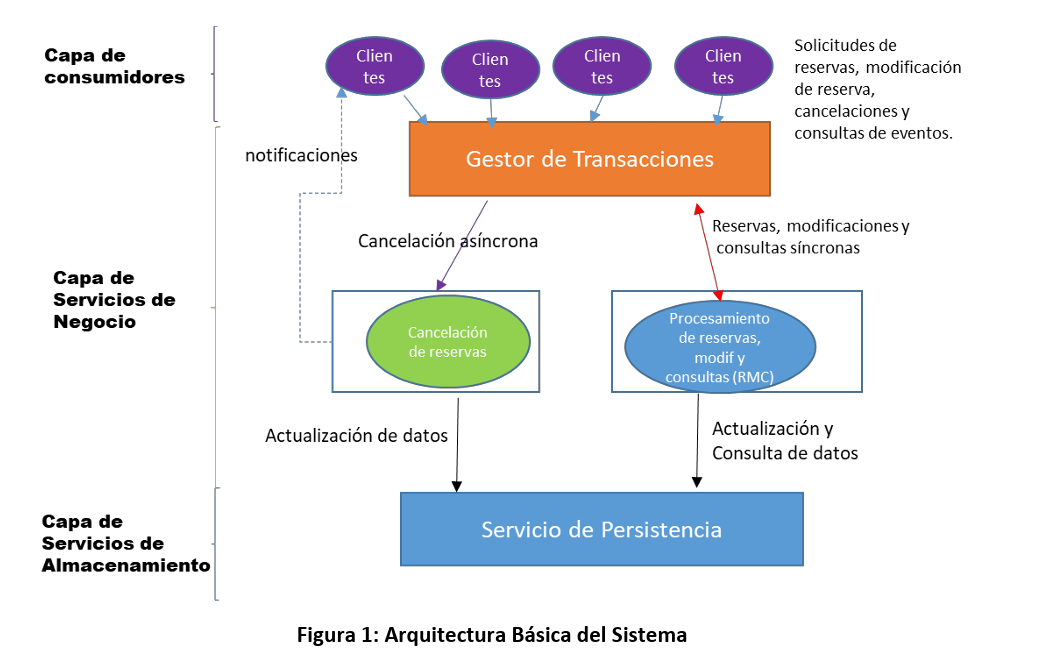
\includegraphics[width=0.92\textwidth]{figuras/arquitectura-basica.png}
    \caption{Arquitectura básica del sistema (Figura~1 del enunciado).}
    \label{fig:arquitectura-basica}
\end{figure}

\begin{itemize}
    \item \textbf{Clientes} (capa de consumidores): envían solicitudes de consulta,
          reserva, modificación y cancelación, y reciben notificaciones.
    \item \textbf{Gestor de Transacciones}: único punto de entrada de la capa de
          negocio. Las operaciones síncronas las envía al procesamiento RMC; las
          cancelaciones las publica para que se apliquen de forma asíncrona.
    \item \textbf{Procesamiento de reservas, modificaciones y consultas (RMC)}:
          valida y ejecuta las operaciones síncronas contra persistencia.
    \item \textbf{Cancelación de reservas}: aplica las cancelaciones y notifica al
          estudiante (línea punteada de la figura).
    \item \textbf{Servicio de Persistencia} (capa de almacenamiento): guarda los
          datos y aplica cada cambio de forma atómica.
\end{itemize}

\subsection{Comunicación entre componentes}

Toda la comunicación usa ZeroMQ (libzmq 4.3 con el enlace C++ cppzmq~\cite{cppzmq}).
La Tabla~\ref{tab:sockets} resume los sockets.

\begin{table}[H]
\centering
\caption{Sockets ZeroMQ de la arquitectura base.}
\label{tab:sockets}
\begin{tabularx}{\textwidth}{p{3.5cm}p{3.2cm}p{1.2cm}Y}
\toprule
Enlace & Sockets & Puerto & Uso \\
\midrule
Cliente $\rightarrow$ Gestor & \codigo{REQ} $\rightarrow$ \codigo{ROUTER} & 5555 &
Todas las solicitudes del estudiante; el cliente espera la respuesta. \\
Gestor $\leftrightarrow$ RMC & \codigo{ROUTER} $\leftrightarrow$ \codigo{DEALER} & 5556 &
El gestor reparte las peticiones entre los procesadores libres (patrón
\emph{load balancing broker}~\cite{zguide}). \\
Gestor $\rightarrow$ Cancelación & \codigo{PUB} $\rightarrow$ \codigo{SUB} & 5557 &
Aviso de cancelación aceptada (tema \codigo{cancelacion}). \\
Cancelación $\rightarrow$ Cliente & \codigo{PUB} $\rightarrow$ \codigo{SUB} & 5558 &
Notificación del resultado; cada cliente se suscribe al tema de su
\codigo{idEstudiante}. \\
RMC / Cancelación $\rightarrow$ Persistencia & \codigo{REQ} $\rightarrow$ \codigo{REP} & 5560 &
Consultas y cambios de datos. \\
\bottomrule
\end{tabularx}
\end{table}

\paragraph{Formato de los mensajes.} Cada mensaje es una trama de texto: la primera
línea es el tipo de operación y las siguientes son pares \codigo{clave=valor}; una
línea \codigo{--} abre una fila nueva para las respuestas con listas. Los errores
se responden con el tipo \codigo{ERROR} y los campos \codigo{codigo} y
\codigo{detalle}.

\begin{minipage}[t]{0.47\textwidth}
\begin{lstlisting}[title={Petición}]
reservar
idSolicitud=S-5f3a9c0d12e4b7a1
idEstudiante=EST-1
idFecha=F-1
cupos=2
\end{lstlisting}
\end{minipage}\hfill
\begin{minipage}[t]{0.47\textwidth}
\begin{lstlisting}[title={Respuesta}]
OK
idReserva=R-1
cupos=2
monto=0
disponibles=298
\end{lstlisting}
\end{minipage}

\subsection{Operaciones}

\begin{table}[H]
\centering
\caption{Operaciones del sistema.}
\label{tab:operaciones}
\small
\begin{tabularx}{\textwidth}{p{3.7cm}p{1.6cm}p{4.5cm}Y}
\toprule
Operación & Tipo & Operación en persistencia & Resultado \\
\midrule
\codigo{consultarEventosMes} & Síncrona & \codigo{listarFechasMes} &
Fechas del mes con evento, lugar, precio, límite, reservas y cupos disponibles. \\
\codigo{consultarReservas} & Síncrona & \codigo{listarReservasEstudiante} &
Reservas del estudiante y su estado. \\
\codigo{reservar} & Síncrona & \codigo{crearReserva} &
Reserva creada (\codigo{idReserva}, cupos, monto, disponibles). \\
\codigo{modificarReserva} & Síncrona & \codigo{modificarReserva} &
Nueva cantidad de cupos y/o fecha; diferencia de precio. \\
\codigo{cancelarReserva} & Asíncrona & \codigo{registrarCancelacion},
\codigo{aplicarCancelacion} & Respuesta inmediata \codigo{EN\_PROCESO}; luego
notificación \codigo{CONFIRMADA} o \codigo{FALLIDA}. \\
\bottomrule
\end{tabularx}
\end{table}

\paragraph{Reglas de negocio.} El límite de cupos de un evento es la capacidad de su
lugar (edificio o teatro registrado) o una capacidad definida a mano para lugares
externos. Las reservas de una fecha nunca superan ese límite; un estudiante tiene
como máximo una reserva activa por evento; las reservas y modificaciones se
aplican completas o no se aplican. Los códigos de error son:

\begin{itemize}\sloppy
    \item \textbf{de negocio:} \codigo{CUPOS\_INSUFICIENTES}, \codigo{RESERVA\_DUPLICADA},
          \codigo{FECHA\_NO\_EXISTE}, \codigo{ESTUDIANTE\_NO\_REGISTRADO},
          \codigo{RESERVA\_AJENA}, \codigo{CANCELACION\_PENDIENTE},
          \codigo{DATOS\_INVALIDOS};
    \item \textbf{técnicos:} \codigo{PERSISTENCIA\_NO\_DISPONIBLE},
          \codigo{SIN\_PROCESADORES}.
\end{itemize}

% =====================================================================
\subsection{Diagrama de despliegue}
\label{sec:despliegue}

La arquitectura base se despliega en las cuatro máquinas del laboratorio. Cada
máquina corre los ejecutables de una parte de la Figura~\ref{fig:arquitectura-basica};
los enlaces indican el protocolo y los puertos.

\begin{figure}[H]
    \centering
    \resizebox{\textwidth}{!}{% Diagrama de despliegue UML – arquitectura base
\begin{tikzpicture}[
    font=\small,
    artefacto/.style={draw, fill=white, rounded corners=1pt, minimum width=4.8cm,
                      minimum height=1.05cm, align=center, inner sep=3pt},
    archivo/.style={artefacto, fill=gris!8},
    titulo/.style={align=center, inner sep=2pt},
    maquina/.style={draw, thick, fill=azulclaro, inner sep=0.3cm},
    enlace/.style={thick, draw=azul},
    etiqueta/.style={font=\scriptsize, fill=white, align=center, inner sep=1.5pt},
]
    % Dibuja el efecto 3D de un nodo UML
    \newcommand{\cubo}[1]{%
        \draw[thick, fill=azulclaro!60] (#1.north west) -- ++(0.3,0.3) -- ($(#1.north east)+(0.3,0.3)$)
            -- ($(#1.south east)+(0.3,0.3)$) -- (#1.south east) -- (#1.north east) -- cycle;
        \draw[thick] (#1.north east) -- ++(0.3,0.3);}

    % ---------------- Máquina 1: clientes
    \node[titulo] (t1) at (0,0) {\guillemotleft device\guillemotright\\\textbf{Máquina 1 – Clientes}};
    \node[artefacto, below=0.2cm of t1] (cli1) {\guillemotleft artifact\guillemotright\\\codigo{bin/cliente} (estudiante 1)};
    \node[artefacto, below=0.25cm of cli1] (cli2) {\guillemotleft artifact\guillemotright\\\codigo{bin/cliente} (estudiante 2)};
    \node[below=0.02cm of cli2] (clin) {\Large $\vdots$};
    \node[artefacto, below=0.02cm of clin] (cli3) {\guillemotleft artifact\guillemotright\\\codigo{bin/cliente} (estudiante N)};

    % ---------------- Máquina 2: gestor
    \node[titulo] (t2) at (9.5,0) {\guillemotleft device\guillemotright\\\textbf{Máquina 2 – Gestor}};
    \node[artefacto, below=0.2cm of t2] (ges) {\guillemotleft artifact\guillemotright\\\codigo{bin/gestor-transacciones}};

    % ---------------- Máquina 3: procesos de negocio
    \node[titulo] (t3) at (9.5,-4.4) {\guillemotleft device\guillemotright\\\textbf{Máquina 3 – Negocio}};
    \node[artefacto, below=0.2cm of t3] (rmc) {\guillemotleft artifact\guillemotright\\\codigo{bin/procesador-rmc}};
    \node[artefacto, below=0.25cm of rmc] (can) {\guillemotleft artifact\guillemotright\\\codigo{bin/cancelacion-reservas}};

    % ---------------- Máquina 4: persistencia
    \node[titulo] (t4) at (9.5,-10.2) {\guillemotleft device\guillemotright\\\textbf{Máquina 4 – Almacenamiento}};
    \node[artefacto, below=0.2cm of t4] (per) {\guillemotleft artifact\guillemotright\\\codigo{bin/persistencia}};
    \node[archivo, below=0.25cm of per] (bit) {\guillemotleft file\guillemotright\\\codigo{datos/bitacora.txt}};

    \begin{scope}[on background layer]
        \node[maquina, fit=(t1)(cli1)(cli3)] (m1) {};
        \node[maquina, fit=(t2)(ges)] (m2) {};
        \node[maquina, fit=(t3)(rmc)(can)] (m3) {};
        \node[maquina, fit=(t4)(per)(bit)] (m4) {};
        \cubo{m1} \cubo{m2} \cubo{m3} \cubo{m4}
    \end{scope}

    % ---------------- Enlaces de red
    \draw[enlace] (m2.west) -- node[etiqueta, above=3pt] {\guillemotleft TCP / ZeroMQ\guillemotright\\REQ $\rightarrow$ ROUTER :5555} (m2.west -| m1.east);
    \draw[enlace] (m2.south) -- node[etiqueta, right=3pt] {\guillemotleft TCP / ZeroMQ\guillemotright\\ROUTER :5556 $\leftrightarrow$ DEALER\\PUB :5557 $\rightarrow$ SUB} (m3.north);
    \draw[enlace] (m3.south) -- node[etiqueta, right=3pt] {\guillemotleft TCP / ZeroMQ\guillemotright\\REQ $\rightarrow$ REP :5560} (m4.north);
    \draw[enlace, dashed] (m3.west) -| node[etiqueta, pos=0.3, below=3pt] {\guillemotleft TCP / ZeroMQ\guillemotright\\notificaciones\\PUB :5558 $\rightarrow$ SUB} (m1.south);
\end{tikzpicture}
}
    \caption{Diagrama de despliegue de la arquitectura base.}
    \label{fig:despliegue}
\end{figure}

% =====================================================================
\subsection{Diagrama de componentes}

Cada componente ofrece y requiere interfaces ZeroMQ. El símbolo de bola indica la
interfaz que un componente provee y el de semicírculo la que otro requiere.

\begin{figure}[H]
    \centering
    \resizebox{!}{0.62\textheight}{% Diagrama de componentes UML – arquitectura base
\begin{tikzpicture}[
    font=\small,
    componente/.style={draw, thick, fill=white, minimum width=4.4cm, minimum height=1.5cm,
                       align=center, inner sep=4pt},
    capa/.style={draw=gris, dashed, rounded corners=4pt, inner sep=0.45cm},
    nombrecapa/.style={font=\footnotesize\bfseries, text=gris, anchor=north west},
    interfaz/.style={font=\scriptsize, align=center, fill=white, inner sep=1pt},
]
    % Icono de componente UML en la esquina superior derecha del nodo
    \newcommand{\icono}[1]{%
        \draw[fill=white] ($(#1.north east)+(-0.55,-0.18)$) rectangle ++(0.36,-0.42);
        \draw[fill=white] ($(#1.north east)+(-0.63,-0.27)$) rectangle ++(0.16,-0.08);
        \draw[fill=white] ($(#1.north east)+(-0.63,-0.44)$) rectangle ++(0.16,-0.08);}
    % Conector de ensamblaje vertical: #1 requiere (arriba), #2 provee (abajo), #3 punto, #4 nombre
    \newcommand{\ensambleV}[4]{%
        \draw[thick] (#2) -- (#3);
        \draw[thick, fill=white] (#3) circle (0.14);
        \draw[thick] (#1) -- ($(#3)+(0,0.26)$);
        \draw[thick] ($(#3)+(0.26,0)$) arc (0:180:0.26);
        \node[interfaz, right=0.32cm of #3] {#4};}

    % ---------------- Consumidores
    \node[componente, fill=morado!12] (cli) at (0,0)
        {\guillemotleft component\guillemotright\\\textbf{Cliente}\\\scriptsize \codigo{Cliente}, \codigo{ConsolaCliente}};

    % ---------------- Negocio
    \node[componente, fill=naranja!20] (ges) at (0,-3.6)
        {\guillemotleft component\guillemotright\\\textbf{Gestor de Transacciones}\\\scriptsize \codigo{GestorTransacciones}};
    \node[componente, fill=azul!15] (rmc) at (-3.4,-7.4)
        {\guillemotleft component\guillemotright\\\textbf{Procesamiento RMC}\\\scriptsize \codigo{ProcesadorRMC}};
    \node[componente, fill=verde!25] (can) at (3.4,-7.4)
        {\guillemotleft component\guillemotright\\\textbf{Cancelación de reservas}\\\scriptsize \codigo{ServicioCancelacion}};

    % ---------------- Almacenamiento
    \node[componente, fill=azul!25, minimum width=6.5cm] (per) at (0,-11.4)
        {\guillemotleft component\guillemotright\\\textbf{Servicio de Persistencia}\\\scriptsize \codigo{ServicioPersistencia}, \codigo{BaseDatos}, \codigo{Almacenamiento}};

    \foreach \c in {cli, ges, rmc, can, per} {\icono{\c}}

    % ---------------- Interfaces
    % Cliente requiere ISolicitudes (provista por el gestor)
    \coordinate (i1) at (0,-1.85);
    \ensambleV{cli.south}{ges.north}{i1}{\codigo{ISolicitudes}\\ROUTER :5555};

    % Gestor requiere IProcesamiento (provista por los procesadores RMC)
    \coordinate (i2) at (-3.4,-5.6);
    \draw[thick] (rmc.north) -- (i2);
    \draw[thick, fill=white] (i2) circle (0.14);
    \draw[thick] (ges.south west) ++(0.8,0) |- ($(i2)+(0,0.9)$) -- ($(i2)+(0,0.26)$);
    \draw[thick] ($(i2)+(0.26,0)$) arc (0:180:0.26);
    \node[interfaz, left=0.32cm of i2] {\codigo{IProcesamiento}\\ROUTER :5556 / DEALER};

    % Cancelación requiere IAvisosCancelacion (provista por el gestor, PUB)
    \coordinate (i3) at (3.4,-5.6);
    \draw[thick] (ges.south east) ++(-0.8,0) |- ($(i3)+(0,0.9)$) -- (i3);
    \draw[thick, fill=white] (i3) circle (0.14);
    \draw[thick] (can.north) -- ($(i3)+(0,-0.26)$);
    \draw[thick] ($(i3)+(-0.26,0)$) arc (180:360:0.26);
    \node[interfaz, right=0.32cm of i3] {\codigo{IAvisosCancelacion}\\PUB :5557 / SUB};

    % Cliente requiere INotificaciones (provista por cancelación, PUB)
    \coordinate (i4) at (6.6,0);
    \draw[thick, dashed] (can.east) -| (i4);
    \draw[thick, fill=white] (i4) circle (0.14);
    \draw[thick, dashed] (cli.east) -- ($(i4)+(-0.26,0)$);
    \draw[thick] ($(i4)+(0,0.26)$) arc (90:270:0.26);
    \node[interfaz, above=0.3cm of i4] {\codigo{INotificaciones}\\PUB :5558 / SUB};

    % RMC y cancelación requieren IPersistencia
    \coordinate (i5) at (0,-9.6);
    \draw[thick] (per.north) -- (i5);
    \draw[thick, fill=white] (i5) circle (0.14);
    \draw[thick] (rmc.south) |- ($(i5)+(-0.6,0.5)$) -- ($(i5)+(0,0.5)$) -- ($(i5)+(0,0.26)$);
    \draw[thick] (can.south) |- ($(i5)+(0.6,0.5)$) -- ($(i5)+(0,0.5)$);
    \draw[thick] ($(i5)+(0.26,0)$) arc (0:180:0.26);
    \node[interfaz, right=0.32cm of i5] {\codigo{IPersistencia}\\REP :5560};

    % ---------------- Capas
    \begin{scope}[on background layer]
        \node[capa, fit=(cli)] (c1) {};
        \node[nombrecapa] at (c1.north west) {Capa de consumidores};
        \node[capa, fit=(ges)(rmc)(can)] (c2) {};
        \node[nombrecapa] at (c2.north west) {Capa de Servicios de Negocio};
        \node[capa, fit=(per)] (c3) {};
        \node[nombrecapa] at (c3.north west) {Capa de Servicios de Almacenamiento};
    \end{scope}
\end{tikzpicture}
}
    \caption{Diagrama de componentes de la arquitectura base.}
    \label{fig:componentes}
\end{figure}

% =====================================================================
\subsection{Diagramas de clases}

El sistema está escrito en C++17 orientado a objetos. La
Figura~\ref{fig:clases-servicios} muestra las clases de los procesos y la
Figura~\ref{fig:clases-dominio} el modelo de dominio que guarda persistencia.
Las decisiones de diseño orientado a objetos más importantes son:

\begin{itemize}
    \item \textbf{Herencia y método plantilla:} \codigo{Servicio::ejecutar()} define el
          ciclo de vida común (señales, \codigo{inicializar}, \codigo{iterar},
          \codigo{finalizar}) y cada proceso implementa sus pasos.
    \item \textbf{Polimorfismo:} \codigo{Lugar} es abstracta; \codigo{LugarUniversidad}
          y \codigo{LugarExterno} calculan la capacidad de forma distinta y
          \codigo{Evento} no necesita saber cuál tiene.
    \item \textbf{Interfaz intercambiable:} \codigo{Almacenamiento} separa la lógica de
          datos de cómo se guardan; hoy es un archivo de bitácora y luego podrá ser
          PostgreSQL sin cambiar \codigo{BaseDatos}.
    \item \textbf{Encapsulamiento:} las reglas de cupos viven en \codigo{FechaEvento}
          y las de estado en \codigo{Reserva} y \codigo{SolicitudCancelacion}.
    \item \textbf{Reutilización:} \codigo{ClienteConfiable} implementa el patrón
          \emph{Lazy Pirate} una sola vez y lo usan el cliente y los procesos de negocio.
\end{itemize}

\begin{sidewaysfigure}
    \centering
    \resizebox{\linewidth}{!}{% Diagrama de clases UML – procesos, comunicación y almacenamiento
\begin{tikzpicture}[font=\footnotesize]
    % ---------------- Clase base de los procesos servidores
    \begin{abstractclass}[text width=6.2cm]{Servicio}{11.2,0}
        \attribute{- nombre : string}
        \attribute{- contexto : zmq::context\_t}
        \operation{+ ejecutar() : int}
        \operation[0]{\# inicializar() : void}
        \operation[0]{\# iterar() : void}
        \operation{\# finalizar() : void}
    \end{abstractclass}

    % ---------------- Procesos
    \begin{class}[text width=6.6cm]{GestorTransacciones}{0,-5.2}
        \inherit{Servicio}
        \attribute{- frontend : socket ROUTER}
        \attribute{- backend : socket ROUTER}
        \attribute{- publicador : socket PUB}
        \attribute{- procesadoresLibres : deque<string>}
        \attribute{- ultimoContacto : map<string,long>}
        \operation{- atenderCliente() : void}
        \operation{- atenderProcesador() : void}
        \operation{- enviarAProcesador(...) : bool}
        \operation{- publicarCancelacion(Mensaje) : void}
    \end{class}

    \begin{class}[text width=6.6cm]{ProcesadorRMC}{7.4,-5.2}
        \inherit{Servicio}
        \attribute{- gestor : socket DEALER}
        \operation{- procesar(Mensaje) : Mensaje}
        \operation{- consultarEventosMes(Mensaje) : Mensaje}
        \operation{- reservar(Mensaje) : Mensaje}
        \operation{- modificarReserva(Mensaje) : Mensaje}
        \operation{- cancelarReserva(Mensaje) : Mensaje}
        \operation{- enviarLatido() : void}
    \end{class}

    \begin{class}[text width=5.8cm]{ServicioCancelacion}{14.6,-5.2}
        \inherit{Servicio}
        \attribute{- avisos : socket SUB}
        \attribute{- notificaciones : socket PUB}
        \operation{- procesar(idSolicitud) : void}
        \operation{- barrer() : void}
        \operation{- notificar(Mensaje) : void}
    \end{class}

    \begin{class}[text width=5.6cm]{ServicioPersistencia}{21.4,-5.2}
        \inherit{Servicio}
        \attribute{- socket : socket REP}
        \operation{- atender(Mensaje) : Mensaje}
        \operation{- aplicar(Mensaje) : Mensaje}
    \end{class}

    % ---------------- Apoyo
    \begin{class}[text width=6.8cm]{ClienteConfiable}{10.9,-12.2}
        \attribute{- endpoint : string}
        \attribute{- timeout : milliseconds}
        \attribute{- intentos : int}
        \attribute{- socket : socket REQ}
        \operation{+ solicitar(Mensaje) : optional<Mensaje>}
    \end{class}

    \begin{class}[text width=6.6cm]{BaseDatos}{18.6,-12.2}
        \operation{+ listarFechasMes(Mensaje) : Mensaje}
        \operation{+ listarReservasEstudiante(Mensaje) : Mensaje}
        \operation{+ crearReserva(Mensaje) : Mensaje}
        \operation{+ modificarReserva(Mensaje) : Mensaje}
        \operation{+ registrarCancelacion(Mensaje) : Mensaje}
        \operation{+ aplicarCancelacion(Mensaje) : Mensaje}
        \operation{+ respuestaPrevia(clave) : Mensaje*}
    \end{class}

    \begin{interface}[text width=5.2cm]{Almacenamiento}{25.4,-12.2}
        \operation[0]{+ cargar() : vector<Mensaje>}
        \operation[0]{+ registrar(Mensaje) : void}
    \end{interface}

    \begin{class}[text width=5.2cm]{AlmacenamientoArchivo}{25.4,-16.2}
        \implement{Almacenamiento}
        \attribute{- ruta : string}
    \end{class}

    \begin{class}[text width=6.4cm]{Mensaje}{2.4,-12.2}
        \attribute{- tipo : string}
        \attribute{- campos : map<string,string>}
        \attribute{- filas : vector<Fila>}
        \operation{+ poner(clave, valor) : Mensaje\&}
        \operation{+ texto(clave) : string}
        \operation{+ serializar() : string}
        \operation{+ deserializar(string) : Mensaje}
    \end{class}

    % ---------------- Consumidores
    \begin{class}[text width=6.6cm]{Cliente}{2.4,-18.0}
        \attribute{- idEstudiante : string}
        \operation{+ consultarEventosMes(mes) : Mensaje}
        \operation{+ reservar(idFecha, cupos) : Mensaje}
        \operation{+ modificarReserva(...) : Mensaje}
        \operation{+ cancelarReserva(idReserva) : Mensaje}
        \operation{+ notificacionesPendientes() : vector}
    \end{class}

    \begin{class}[text width=4.4cm]{ConsolaCliente}{10.9,-18.8}
        \operation{+ ejecutar() : int}
    \end{class}

    % ---------------- Relaciones
    \composition{ProcesadorRMC}{}{}{ClienteConfiable}
    \composition{ServicioCancelacion}{}{}{ClienteConfiable}
    \composition{ServicioPersistencia}{}{}{BaseDatos}
    \aggregation{ServicioPersistencia}{}{}{Almacenamiento}
    \composition{Cliente}{}{}{ClienteConfiable}
    \unidirectionalAssociation{ConsolaCliente}{usa}{1}{Cliente}
    \draw[umlcd style dashed line, ->] (GestorTransacciones) -- node[left, font=\scriptsize] {\guillemotleft use\guillemotright} (Mensaje);
\end{tikzpicture}
}
    \caption{Diagrama de clases de los procesos y la comunicación.}
    \label{fig:clases-servicios}
\end{sidewaysfigure}

\begin{sidewaysfigure}
    \centering
    \resizebox{\linewidth}{!}{% Diagrama de clases UML – modelo de dominio (capa de almacenamiento)
\begin{tikzpicture}[font=\footnotesize]
    \begin{abstractclass}[text width=4.4cm]{Lugar}{0,0}
        \operation[0]{+ capacidad() : int}
        \operation[0]{+ descripcion() : string}
    \end{abstractclass}

    \begin{class}[text width=4.4cm]{LugarUniversidad}{-2.6,-4.6}
        \inherit{Lugar}
        \attribute{- id : string}
        \attribute{- nombre : string}
        \attribute{- tipo : EDIFICIO | TEATRO}
        \attribute{- capacidad : int}
    \end{class}

    \begin{class}[text width=4.0cm]{LugarExterno}{2.6,-4.6}
        \inherit{Lugar}
        \attribute{- direccion : string}
        \attribute{- capacidad : int}
    \end{class}

    \begin{class}[text width=4.6cm]{Evento}{8.4,0}
        \attribute{- id : string}
        \attribute{- nombre : string}
        \attribute{- precio : long}
        \operation{+ limite() : int}
    \end{class}

    \begin{class}[text width=5.4cm]{FechaEvento}{8.4,-5.6}
        \attribute{- id : string}
        \attribute{- fecha : string}
        \attribute{- reservas : int}
        \operation{+ mes() : string}
        \operation{+ hayCupo(cupos, limite) : bool}
        \operation{+ ocupar(cupos) : void}
        \operation{+ liberar(cupos) : void}
    \end{class}

    \begin{class}[text width=5.0cm]{Estudiante}{14.8,0}
        \attribute{- codigo : string}
        \attribute{- nombre : string}
        \attribute{- tipoDocumento : string}
        \attribute{- numeroDocumento : string}
        \attribute{- carrera : string}
        \attribute{- departamento : string}
        \attribute{- semestre : int}
        \attribute{- correo : string}
        \attribute{- telefono : string}
    \end{class}

    \begin{class}[text width=5.4cm]{Reserva}{14.8,-7.0}
        \attribute{- id : string}
        \attribute{- cupos : int}
        \attribute{- estado : ACTIVA | CANCELADA}
        \operation{+ cambiar(cupos, idFecha) : void}
        \operation{+ cancelar() : void}
    \end{class}

    \begin{class}[text width=6.4cm]{Transaccion}{22.4,-7.0}
        \attribute{- id : string}
        \attribute{- idSolicitud : string}
        \attribute{- tipo : RESERVA | MODIFICACION | CANCELACION}
        \attribute{- cupos : int}
        \attribute{- monto : long}
        \attribute{- instante : long}
    \end{class}

    \begin{class}[text width=6.4cm]{SolicitudCancelacion}{22.4,0}
        \attribute{- idSolicitud : string}
        \attribute{- estado : PENDIENTE | CONFIRMADA | FALLIDA}
        \attribute{- creada : long}
        \operation{+ confirmar() : void}
        \operation{+ fallar(detalle) : void}
    \end{class}

    \unidirectionalAssociation{Evento}{se realiza en}{1}{Lugar}
    \composition{Evento}{fechas}{1..*}{FechaEvento}
    \association{Estudiante}{}{1}{Reserva}{reservas}{0..*}
    \unidirectionalAssociation{Reserva}{fecha}{1}{FechaEvento}
    \association{Reserva}{}{1}{Transaccion}{historial}{1..*}
    \unidirectionalAssociation{SolicitudCancelacion}{cancela}{1}{Reserva}
\end{tikzpicture}
}
    \caption{Diagrama de clases del modelo de dominio.}
    \label{fig:clases-dominio}
\end{sidewaysfigure}
\clearpage

% =====================================================================
\subsection{Diagramas de secuencia}

\paragraph{Consultar los eventos de un mes.} El gestor entrega la petición a un
procesador RMC libre, que valida el mes y pide a persistencia las fechas.

\begin{figure}[H]
    \centering
    \secuenciaConsultar
    \caption{Secuencia: consultar los eventos de un mes.}
\end{figure}

\paragraph{Reservar.} Persistencia revisa primero si el \codigo{idSolicitud} ya se
procesó (reintento); si no, valida todo y aplica el cambio de forma atómica.

\begin{figure}[H]
    \centering
    \resizebox{\textwidth}{!}{\secuenciaReservar}
    \caption{Secuencia: reservar cupos.}
\end{figure}

\paragraph{Modificar una reserva.} Igual que la reserva, pero libera los cupos de la
fecha original y ocupa los de la fecha destino en una sola operación.

\begin{figure}[H]
    \centering
    \resizebox{\textwidth}{!}{\secuenciaModificar}
    \caption{Secuencia: modificar una reserva.}
\end{figure}

\paragraph{Cancelar una reserva (asíncrona).} La solicitud se guarda como
\codigo{PENDIENTE} \emph{antes} de responder; así, aunque el aviso PUB/SUB se
pierda, el barrido periódico la encuentra y la aplica. El estudiante recibe de
inmediato \codigo{EN\_PROCESO} y después la notificación con el resultado.

\begin{figure}[H]
    \centering
    \resizebox{\textwidth}{!}{\secuenciaCancelar}
    \caption{Secuencia: cancelar una reserva (asíncrona).}
\end{figure}

\section{Componentes para escalabilidad y tolerancia a fallos}
\label{sec:escalabilidad}

La arquitectura base tiene una sola instancia de cada componente: es simple, pero
el gestor, el servicio de cancelación y persistencia son puntos únicos de fallo, y
el procesamiento de un único procesador RMC limita el número de transacciones por
minuto. Para la segunda entrega se incorporarán los componentes de la
Tabla~\ref{tab:componentes-ft}. Aquí solo se mencionan y justifican; los diagramas
completos se presentarán en esa entrega.

\begin{longtable}{p{3.6cm}p{4.4cm}p{7.3cm}}
\caption{Componentes de escalabilidad y tolerancia a fallos.}
\label{tab:componentes-ft}\\
\toprule
Componente & Qué resuelve & Justificación \\
\midrule
\endfirsthead
\toprule
Componente & Qué resuelve & Justificación \\
\midrule
\endhead
\textbf{Réplicas del procesador RMC} &
Escalabilidad horizontal de reservas, modificaciones y consultas. &
Los procesadores no guardan estado, así que cualquier réplica atiende cualquier
petición. El gestor ya reparte la carga entre los procesadores libres, de modo que
agregar réplicas no cambia el código. Es la diferencia principal entre la
arquitectura base y la escalable en las pruebas de la Tabla~1. \\
\textbf{Clientes \emph{Lazy Pirate}} &
Peticiones o respuestas perdidas; procesos caídos. &
Cada cliente espera con timeout y, si no hay respuesta, cierra el socket, abre
otro y reenvía la misma petición~\cite{zguide}. Funciona porque las operaciones
son idempotentes por \codigo{idSolicitud}. \\
\textbf{Latidos \emph{Paranoid Pirate}} &
Detectar procesadores caídos sin esperar a que falle una petición. &
Gestor y procesadores intercambian latidos cada 1\,s; tres perdidos sacan al
procesador del grupo. Si el gestor se reinicia, los procesadores se registran de
nuevo solos. \\
\textbf{Broker Majordomo} &
Más servicios y réplicas sin configuración manual. &
El protocolo Majordomo~\cite{rfc7} generaliza el gestor: los procesos se
registran por nombre de servicio (por ejemplo \codigo{rmc}, \codigo{persistencia})
y el broker enruta y balancea. Permite poner también varias réplicas de
persistencia detrás de un broker. \\
\textbf{Par \emph{Binary Star} para el gestor} &
El gestor deja de ser punto único de fallo. &
Un gestor primario y uno de respaldo en máquinas distintas se vigilan con
latidos; si el primario cae, el respaldo toma el control y los clientes
(\emph{Lazy Pirate}) cambian de dirección. El gestor no guarda datos de negocio,
así que el cambio no pierde información. \\
\textbf{Guardar primero y luego publicar + barrido} &
Avisos PUB/SUB perdidos; caída del servicio de cancelación. &
ZeroMQ PUB/SUB no es durable. La solicitud se guarda como \codigo{PENDIENTE}
antes de responder y un barrido cada 2\,s aplica las que no recibieron aviso.
Varias réplicas del servicio de cancelación pueden trabajar a la vez porque
persistencia aplica cada solicitud una sola vez. \\
\textbf{Base de datos replicada (PostgreSQL con CloudNativePG)} &
Persistencia deja de ser punto único de fallo; más capacidad de lectura. &
Una instancia primaria y réplicas con replicación síncrona: si la primaria cae se
promueve una réplica sin perder confirmaciones (RPO = 0). Las consultas pueden
leer de las réplicas y las reservas siempre se deciden en la primaria. La interfaz
\codigo{Almacenamiento} permite cambiar la bitácora por PostgreSQL. \\
\textbf{Kubernetes (1 plano de control + 3 workers)} &
Reinicio automático, reparto de réplicas y escalado. &
Reinicia los procesos caídos (sondas de \emph{liveness}), reparte las réplicas
en nodos distintos (anti-afinidad), reubica los procesos de un nodo caído y
puede escalar los procesadores según la carga (\emph{HorizontalPodAutoscaler}). \\
\textbf{Idempotencia y operaciones atómicas} &
Reintentos sin duplicados; nada aplicado a medias. &
Ya está en el diseño base: cada cambio se valida completo antes de aplicarse y
se guarda con su \codigo{idSolicitud}. Es lo que hace seguros todos los
reintentos anteriores. \\
\textbf{Monitoreo (Prometheus y Grafana)} &
Detectar degradación y fallos. &
Alertas cuando el p95 supera 1\,s, crece la tasa de errores o hay cancelaciones
pendientes antiguas; sirve también para las pruebas de desempeño. \\
\textbf{Seguridad (CurveZMQ y autenticación)} &
Confidencialidad e integridad de los mensajes. &
Cifrado autenticado de todos los sockets y verificación de identidad del
estudiante (sección~\ref{sec:modelos}). \\
\bottomrule
\end{longtable}

\paragraph{Arquitectura escalable para las pruebas.} Para comparar con la base en
las pruebas de la Tabla~1 se usarán las mismas máquinas y programas, cambiando solo
la cantidad de réplicas:

\begin{table}[H]
\centering
\caption{Arquitectura base frente a escalable.}
\begin{tabular}{lcc}
\toprule
Componente & Base & Escalable \\
\midrule
Gestor de Transacciones & 1 & 1 (+ respaldo \emph{Binary Star}) \\
Procesador RMC & 1 & 3 (uno por máquina de servicios) \\
Servicio de cancelación & 1 & 2 \\
Persistencia & 1 & 1 primaria + réplica \\
\bottomrule
\end{tabular}
\end{table}

Se espera que la escalable aumente las transacciones por minuto y reduzca el
tiempo de respuesta cuando hay más clientes, porque en la base todas las
peticiones esperan en la cola de un único procesador RMC.

\section{Protocolo de pruebas}
\label{sec:pruebas}

El protocolo cubre los tipos de prueba de un sistema informático, desde las piezas
aisladas hasta el sistema completo bajo carga y fallos. Las pruebas se ejecutan en
este orden: si un nivel falla, no se avanza al siguiente.

\subsection{Tipos de prueba, herramientas y criterios}

\begin{longtable}{p{3.0cm}p{5.6cm}p{3.2cm}p{3.5cm}}
\caption{Tipos de prueba.}\\
\toprule
Tipo & Qué verifica & Herramientas & Cuándo \\
\midrule
\endfirsthead
\toprule
Tipo & Qué verifica & Herramientas & Cuándo \\
\midrule
\endhead
Análisis estático & Errores de programación sin ejecutar: variables sin usar,
conversiones peligrosas, estilo. & \codigo{g++ -Wall -Wextra}, \codigo{cppcheck},
\codigo{clang-tidy} & En cada compilación \\
Unitarias & Cada clase por separado: \codigo{Mensaje} (serializar y deserializar),
\codigo{FechaEvento} (\codigo{hayCupo}), \codigo{BaseDatos} (reglas de reserva),
\codigo{AlmacenamientoArchivo} (bitácora). & GoogleTest & En cada cambio \\
Integración & Dos componentes reales juntos: RMC $\leftrightarrow$ persistencia,
gestor $\leftrightarrow$ RMC, reconstrucción desde la bitácora. & GoogleTest + procesos
reales en una máquina & En cada cambio \\
Protocolo (contrato) & Cada proceso envía y acepta exactamente las tramas y campos
acordados; errores ante mensajes mal formados. & Cliente de prueba con cppzmq & En
cada cambio \\
Funcionales (extremo a extremo) & Cada requisito funcional a través de las tres
capas (Tabla~\ref{tab:e2e}). & \codigo{bin/cliente} con guiones de entrada + script
\codigo{bash} & Antes de cada entrega \\
Concurrencia y consistencia & Sin sobrecupo, sin reservas duplicadas, contadores
iguales a la suma de reservas. & Varios clientes simultáneos & Antes de cada entrega \\
Regresión & Lo que funcionaba sigue funcionando después de un cambio. & Repetir las
suites anteriores & En cada \emph{merge} a \codigo{develop} \\
Desempeño (Tabla~1) & Tiempo promedio, desviación estándar y TPM de consultas y
reservas con 3, 5 y 8 clientes, base frente a escalable. & Sección~\ref{sec:metricas}
y \ref{sec:carga} & Entrega final \\
Carga, estrés y resistencia & Meta de p95 < 1\,s, punto de saturación y
estabilidad durante horas (fugas de memoria). & Generador de carga, \codigo{pidstat},
Valgrind & Entrega final \\
Escalabilidad & Ganancia de TPM al pasar de 1 a 2 y 3 procesadores RMC. &
Generador de carga & Entrega final \\
Inyección de fallos & Caídas y mensajes perdidos se enmascaran
(Tabla~\ref{tab:fallos}). & \codigo{kill}, \codigo{tc netem}, \codigo{iptables} &
Entrega final \\
Seguridad & Validación de entradas, propiedad de las reservas, repetición de
mensajes, tráfico cifrado. & Cliente de prueba, Wireshark & Entrega final \\
Despliegue e instalación & El sistema se compila y arranca en máquinas limpias
siguiendo el README. & \codigo{make}, scripts, Kubernetes & Antes de cada entrega \\
Aceptación y usabilidad & Un estudiante completa consulta y reserva sin ayuda; los
mensajes son claros. & Sesión guiada con usuarios & Entrega final \\
\bottomrule
\end{longtable}

\subsection{Casos funcionales}

\begin{longtable}{p{1.4cm}p{6.6cm}p{7.3cm}}
\caption{Casos de prueba funcionales de extremo a extremo.}
\label{tab:e2e}\\
\toprule
ID & Caso & Resultado esperado \\
\midrule
\endfirsthead
\toprule
ID & Caso & Resultado esperado \\
\midrule
\endhead
F-01 & Consultar un mes con eventos (\codigo{2026-11}). & Solo fechas de ese mes, en
orden, con lugar, precio, límite, reservas y disponibles. \\
F-02 & Consultar un mes sin eventos. & Lista vacía, sin error. \\
F-03 & Consultar con un mes mal escrito (\codigo{2026-13}). & \codigo{DATOS\_INVALIDOS}. \\
F-04 & Reservar 2 cupos en una fecha con cupo. & Reserva creada; los disponibles
bajan en 2; se registra una transacción. \\
F-05 & Reservar más cupos de los disponibles. & \codigo{CUPOS\_INSUFICIENTES}; nada
cambia. \\
F-06 & Reservar exactamente los cupos restantes y luego uno más. & La primera
funciona; la segunda \codigo{CUPOS\_INSUFICIENTES}. \\
F-07 & Segunda reserva del mismo estudiante en el mismo evento. &
\codigo{RESERVA\_DUPLICADA}. \\
F-08 & Reservar con cupos 0 o negativos, o una fecha inexistente. &
\codigo{DATOS\_INVALIDOS} / \codigo{FECHA\_NO\_EXISTE}. \\
F-09 & Reservar con un estudiante no registrado. & \codigo{ESTUDIANTE\_NO\_REGISTRADO}. \\
F-10 & Modificar cupos y luego fecha de una reserva. & Contadores de ambas fechas
correctos; diferencia de precio calculada. \\
F-11 & Modificar o cancelar la reserva de otro estudiante. & \codigo{RESERVA\_AJENA}. \\
F-12 & Cancelar una reserva. & Respuesta inmediata \codigo{EN\_PROCESO}; después
notificación \codigo{CONFIRMADA} y cupos liberados. \\
F-13 & Modificar una reserva con cancelación pendiente. & \codigo{CANCELACION\_PENDIENTE}. \\
F-14 & Reiniciar persistencia y consultar. & Las reservas anteriores siguen ahí. \\
\bottomrule
\end{longtable}

\subsection{Concurrencia y fallos}

\begin{longtable}{p{1.4cm}p{6.6cm}p{7.3cm}}
\caption{Casos de concurrencia e inyección de fallos.}
\label{tab:fallos}\\
\toprule
ID & Caso & Resultado esperado \\
\midrule
\endfirsthead
\toprule
ID & Caso & Resultado esperado \\
\midrule
\endhead
C-01 & 20 clientes piden 1 cupo a la vez en una fecha con 5 disponibles. & Exactamente 5
reservas; 15 \codigo{CUPOS\_INSUFICIENTES}. \\
C-02 & El mismo \codigo{idSolicitud} enviado 10 veces en paralelo. & Una sola
reserva; 10 respuestas idénticas. \\
C-03 & Al final de cada corrida: suma de cupos de las reservas activas de cada
fecha. & Igual al contador de reservas de la fecha y nunca mayor al límite. \\
FT-01 & Matar un procesador RMC durante una ráfaga de reservas. & Los clientes
reintentan; sin duplicados; el gestor lo descarta en $\le$ 3\,s. \\
FT-02 & Perder la respuesta de \codigo{reservar} (retardo con \codigo{tc netem}
mayor al timeout). & El reintento devuelve la misma reserva, sin duplicado. \\
FT-03 & Reiniciar el gestor con carga. & Los procesadores se vuelven a registrar;
los clientes continúan tras reintentar. \\
FT-04 & Detener el servicio de cancelación y cancelar reservas. & Las solicitudes
quedan \codigo{PENDIENTE}; al volver, el barrido las aplica una vez. \\
FT-05 & Matar persistencia a mitad de la carga y reiniciarla. & Ninguna reserva
aplicada a medias; el estado se reconstruye desde la bitácora. \\
FT-06 & 10\,\% de pérdida de paquetes entre cliente y gestor. & Los reintentos
funcionan; sin duplicados. \\
\bottomrule
\end{longtable}

\subsection{Pruebas de desempeño}

\begin{itemize}
    \item \textbf{Escenarios de la Tabla~1} (sección~\ref{sec:metricas}): 3, 5 y 8
          clientes en las arquitecturas base y escalable.
    \item \textbf{Carga:} subir gradualmente el número de clientes hasta el uso esperado
          y verificar p95 < 1\,s.
    \item \textbf{Estrés:} seguir aumentando clientes hasta que el p95 supere 1\,s o los
          errores superen 1\,\%; se registra el TPM máximo y qué componente se satura.
    \item \textbf{Resistencia:} carga media durante 2 horas; la memoria de los procesos
          no debe crecer sin límite.
    \item \textbf{Escalabilidad:} misma carga con 1, 2 y 3 procesadores RMC; se espera
          que el TPM crezca al agregar réplicas.
\end{itemize}

\subsection{Criterios de aceptación}

\begin{itemize}
    \item Todos los casos funcionales F-01 a F-14 pasan.
    \item Ninguna corrida termina con sobrecupo, reservas duplicadas o contadores
          descuadrados (C-03).
    \item El 95\,\% de las transacciones termina en menos de 1\,s en los escenarios de
          la Tabla~1.
    \item Los fallos FT-01 a FT-06 no producen pérdida ni duplicación de datos.
\end{itemize}

\subsection{Trazabilidad}

\begin{table}[H]
\centering
\caption{Requisitos frente a pruebas.}
\begin{tabularx}{\textwidth}{p{6.4cm}Y}
\toprule
Requisito & Pruebas \\
\midrule
Consultar eventos de un mes & Unitarias de \codigo{BaseDatos}; F-01 a F-03 \\
Reservar sin superar el límite & F-04 a F-09; C-01, C-03 \\
Modificar y cancelar (asíncrona) & F-10 a F-13; FT-04 \\
Reintentos sin duplicados & C-02; FT-01, FT-02, FT-06 \\
Atomicidad y durabilidad & F-14; FT-05 \\
Transacciones < 1\,s y Tabla~1 & Pruebas de desempeño \\
Seguridad & F-11; pruebas de seguridad \\
\bottomrule
\end{tabularx}
\end{table}

\section{Herramientas y estrategia para las métricas de desempeño}
\label{sec:metricas}

\subsection{Escenarios y variables de la Tabla~1}

Cada escenario se ejecuta sobre la arquitectura base y sobre la escalable:

\begin{table}[H]
\centering
\caption{Escenarios de la Tabla~1.}
\begin{tabular}{lcccc}
\toprule
Escenario & Clientes & Solo consultan & Consultan y reservan & Reservan y modifican \\
\midrule
ESC-3 & 3 & 2 & 1 & 0 \\
ESC-5 & 5 & 3 & 0 & 2 \\
ESC-8 & 8 & 4 & 0 & 4 \\
\bottomrule
\end{tabular}
\end{table}

Se miden cuatro variables. Para efectos de la medición, la modificación cuenta
como operación de reserva y también se reporta por separado.

\begin{table}[H]
\centering
\caption{Variables y dónde se miden.}
\begin{tabularx}{\textwidth}{p{4.6cm}p{4.2cm}Y}
\toprule
Variable & Fórmula & Dónde se mide \\
\midrule
Tiempo promedio y desviación estándar de las \textbf{consultas} &
$\bar{t}=\frac{1}{n}\sum t_i$, \ $s=\sqrt{\frac{1}{n-1}\sum (t_i-\bar{t})^2}$ &
En cada cliente: inicio y fin de cada \codigo{consultarEventosMes} con el reloj
monótono (\codigo{std::chrono::steady\_clock}). \\
Tiempo promedio y desviación estándar de las \textbf{reservas} & Igual &
En cada cliente, para \codigo{reservar} y \codigo{modificarReserva}. \\
\textbf{TPM de consultas} & consultas exitosas $\div$ minutos de medición &
En el Gestor de Transacciones: contador por categoría y por minuto. \\
\textbf{TPM de reservas} & reservas confirmadas $\div$ minutos de medición &
En el Gestor y verificado en persistencia: transacciones de la bitácora con
instante dentro de la ventana de medición. \\
\bottomrule
\end{tabularx}
\end{table}

El tiempo de respuesta se mide en el cliente porque es lo que percibe el
estudiante: incluye red, gestor, procesador y persistencia. Las duraciones usan el
reloj monótono de una sola máquina, así que la deriva entre relojes no las afecta.
Las TPM se cuentan en el gestor de transacciones, como permite el enunciado, y se
cruzan con persistencia para confirmar que coinciden.

\subsection{Instrumentación en el código}

\begin{itemize}
    \item \textbf{Cliente de carga:} registra por operación el instante de inicio, la
          categoría (\codigo{CONSULTA} o \codigo{RESERVA}), la operación, la latencia
          en milisegundos, si fue exitosa y el código de error. Al terminar escribe un
          archivo CSV:
\begin{lstlisting}
escenario,arquitectura,cliente,tipo_cliente,inicio_ms,categoria,operacion,latencia_ms,exitosa,codigo_error
ESC-5,base,C1,consulta,1792706556363,CONSULTA,consultarEventosMes,4,1,
\end{lstlisting}
    \item \textbf{Gestor de Transacciones:} una clase \codigo{Metricas} acumula por
          categoría la cantidad, los errores, la suma y la suma de cuadrados de las
          latencias, y cada minuto agrega al archivo
          \codigo{metricas\_gestor.csv} una línea con transacciones, errores,
          promedio, desviación y TPM. Agregar un contador cuesta unos pocos
          nanosegundos, así que no altera lo que se mide.
    \item \textbf{Persistencia:} cada transacción guarda su instante en la bitácora,
          lo que permite contar las reservas confirmadas por minuto.
    \item \textbf{Recursos:} CPU y memoria por proceso con \codigo{pidstat} (paquete
          \codigo{sysstat}) cada segundo, para identificar el cuello de botella.
\end{itemize}

\subsection{Herramientas}

\begin{table}[H]
\centering
\caption{Herramientas y librerías de medición.}
\begin{tabularx}{\textwidth}{p{4.4cm}Y}
\toprule
Herramienta & Uso \\
\midrule
\codigo{std::chrono} (C++17) & Reloj monótono para las latencias y reloj de pared
para ubicar cada medición en la ventana. \\
Archivos CSV & Formato común de los clientes, el gestor y \codigo{pidstat}. \\
Python 3 + \textbf{pandas} y \textbf{NumPy} & Unir los CSV de todos los clientes,
descartar el calentamiento y calcular promedio, desviación estándar muestral, p95,
TPM y porcentaje de transacciones < 1\,s por escenario y arquitectura. \\
\textbf{matplotlib} & Gráficos para el informe. \\
\codigo{pidstat} / \codigo{htop} & Uso de CPU y memoria por proceso. \\
Prometheus + Grafana (segunda entrega) & Paneles en tiempo real con la librería
\textbf{prometheus-cpp} en los procesos, y \codigo{node\_exporter} para las
máquinas. Útiles para las pruebas de estrés y de fallos. \\
\bottomrule
\end{tabularx}
\end{table}

\subsection{Procedimiento de cada corrida}

\begin{enumerate}
    \item Levantar la arquitectura (base: 1 procesador RMC; escalable: 3) con datos
          iniciales limpios.
    \item Lanzar a la vez los procesos cliente del escenario.
    \item Descartar los primeros 2 minutos (calentamiento) y medir durante 10 minutos.
    \item Repetir cada combinación 3 veces y reportar el promedio de las repeticiones.
    \item Verificar la consistencia (C-03): ninguna fecha con sobrecupo.
\end{enumerate}

Son 3 escenarios $\times$ 2 arquitecturas $\times$ 3 repeticiones = 18 corridas.

\subsection{Presentación de los resultados}

Los resultados se presentarán en una tabla con una fila por escenario y
arquitectura (promedio y desviación de consultas y de reservas, TPM de consultas y
de reservas, errores) y en cuatro gráficos con el número de clientes (3, 5 y 8) en
el eje horizontal y una línea por arquitectura:

\begin{enumerate}
    \item tiempo promedio de las consultas, con barras de $\pm$ una desviación estándar;
    \item tiempo promedio de las reservas, con barras de $\pm$ una desviación estándar;
    \item TPM de consultas;
    \item TPM de reservas.
\end{enumerate}

\begin{table}[H]
\centering
\caption{Plantilla de la tabla de resultados (se completará en la entrega final).}
\small
\begin{tabular}{llcccccc}
\toprule
& & \multicolumn{2}{c}{Consultas (ms)} & \multicolumn{2}{c}{Reservas (ms)} & \multicolumn{2}{c}{TPM} \\
\cmidrule(lr){3-4}\cmidrule(lr){5-6}\cmidrule(lr){7-8}
Escenario & Arquitectura & Prom. & Desv. & Prom. & Desv. & Consultas & Reservas \\
\midrule
ESC-3 & Base & & & & & & \\
ESC-3 & Escalable & & & & & & \\
ESC-5 & Base & & & & & & \\
ESC-5 & Escalable & & & & & & \\
ESC-8 & Base & & & & & & \\
ESC-8 & Escalable & & & & & & \\
\bottomrule
\end{tabular}
\end{table}

\section{Generación de carga desde los clientes}
\label{sec:carga}

\subsection{Herramienta}

Se usará un \textbf{generador de carga propio en C++}: el mismo programa cliente
(\codigo{bin/cliente}) con un modo de carga que reutiliza la clase \codigo{Cliente}.
Se descartaron herramientas como JMeter, Locust o k6 porque hablan HTTP y no
ZeroMQ; usarlas obligaría a escribir un adaptador que agregaría su propio tiempo a
las mediciones. Con el cliente propio, la carga recorre exactamente el mismo camino
que un estudiante real.

\begin{lstlisting}
bin/cliente --carga consulta|consulta-reserva|reserva-modificacion
            --duracion 720 --id C1 --escenario ESC-5 --arquitectura base
            --csv resultados/tiempos_ESC-5_base_C1.csv
\end{lstlisting}

\subsection{Método}

\begin{itemize}
    \item \textbf{Un proceso por cliente simulado}, cada uno con su propio socket
          \codigo{REQ}. Así los clientes son realmente concurrentes y no comparten
          colas internas.
    \item \textbf{Ciclo cerrado sin tiempo de espera:} cada cliente envía la siguiente
          solicitud apenas recibe la respuesta. Con pocos clientes (3 a 8) esto mide
          la capacidad real del sistema y da resultados repetibles.
    \item \textbf{Tipos de cliente} según la Tabla~1:
          \begin{itemize}
              \item \emph{consulta}: repite \codigo{consultarEventosMes} sobre los meses con eventos;
              \item \emph{consulta-reserva}: una consulta y luego una reserva de 1 cupo;
              \item \emph{reserva-modificacion}: una reserva y luego su modificación
                    (cambio de cupos).
          \end{itemize}
    \item \textbf{Datos de prueba:} cada reserva la hace un estudiante distinto,
          generado para la prueba, en un evento con capacidad suficiente. Así no se
          choca con la regla de una reserva por evento ni se agotan los cupos, y los
          errores de negocio no contaminan los tiempos.
    \item \textbf{Orquestación:} un script \codigo{bash},
          \codigo{scripts/correr\_escenario.sh}, recibe el escenario
          (\codigo{ESC-3}, \codigo{ESC-5} o \codigo{ESC-8}) y la arquitectura
          (\codigo{base} o \codigo{escalable}), lanza los procesos del escenario al mismo tiempo, espera a que terminen y
          une sus archivos CSV.
    \item \textbf{Ubicación:} los clientes corren en una máquina distinta a la de los
          servicios (Máquina 1 de la Figura~\ref{fig:despliegue}) para no competir por
          CPU con el sistema medido.
    \item \textbf{Pruebas de estrés y resistencia:} el mismo generador, lanzando más
          procesos de forma escalonada.
\end{itemize}

Para la prueba de concurrencia C-01 se lanza un grupo de procesos que envían su
reserva al mismo tiempo sobre una fecha con pocos cupos.

\section{Implementación de la primera entrega}
\label{sec:implementacion}

\subsection{Alcance}

Se implementaron en C++17 orientado a objetos, con ZeroMQ, los componentes de la
arquitectura base con las operaciones de \textbf{consulta de eventos del mes} y
\textbf{reserva de cupos}:

\begin{table}[H]
\centering
\caption{Componentes implementados.}
\begin{tabularx}{\textwidth}{p{3.8cm}p{4.6cm}Y}
\toprule
Componente (Figura~\ref{fig:arquitectura-basica}) & Ejecutable & Clases \\
\midrule
Clientes & \codigo{bin/cliente} & \codigo{Cliente}, \codigo{ConsolaCliente} \\
Gestor de Transacciones & \codigo{bin/gestor-transacciones} & \codigo{GestorTransacciones} \\
Procesamiento RMC & \codigo{bin/procesador-rmc} & \codigo{ProcesadorRMC} \\
Servicio de Persistencia & \codigo{bin/persistencia} & \codigo{ServicioPersistencia},
\codigo{BaseDatos}, \codigo{AlmacenamientoArchivo}, modelo de dominio \\
Común & — & \codigo{Servicio}, \codigo{Mensaje}, \codigo{ClienteConfiable} \\
\bottomrule
\end{tabularx}
\end{table}

El componente de Cancelación de reservas está diseñado (sección~\ref{sec:diseno})
pero no se implementó, porque esta entrega solo incluye consulta y reserva. Aunque
la tolerancia a fallos no se exigía, el código ya incluye los reintentos
\emph{Lazy Pirate}, los latidos entre gestor y procesadores y las reservas
idempotentes, porque son la base de la segunda entrega.

Persistencia guarda los datos en memoria y escribe cada reserva en un archivo de
bitácora antes de responder; al arrancar vuelve a aplicar la bitácora. Arranca con
datos de ejemplo: cuatro eventos en noviembre y diciembre de 2026 (en el Teatro
Mayor, una sala de 5 cupos, un auditorio y un lugar externo) y los estudiantes
\codigo{EST-1}, \codigo{EST-2} y \codigo{EST-3}.

\subsection{Compilación y ejecución}

\begin{lstlisting}
sudo apt install g++ make libzmq3-dev cppzmq-dev
make
scripts/iniciar_sistema.sh base      # o "escalable" (3 procesadores RMC)
bin/cliente EST-1                    # menu: 1 consultar mes, 2 reservar
scripts/detener_sistema.sh
\end{lstlisting}

Para ejecutar en varias máquinas se indican las direcciones con variables de
entorno (\codigo{GESTOR\_ENDPOINT}, \codigo{GESTOR\_BACKEND},
\codigo{PERSISTENCIA\_ENDPOINT}, etc.). El código fuente y el README están en el
repositorio: \repositorio.

\subsection{Verificación realizada}

\begin{itemize}
    \item Consulta del mes \codigo{2026-11}: lista las fechas con cupos y precios.
    \item Errores: fecha inexistente, cupos en 0, mes mal escrito, estudiante no
          registrado y reserva duplicada.
    \item Tres estudiantes pidieron 2 cupos al mismo tiempo en la sala de 5: dos
          reservas se crearon y la tercera recibió \codigo{CUPOS\_INSUFICIENTES}.
    \item Tras reiniciar persistencia, las reservas se conservaron.
\end{itemize}


\begin{thebibliography}{9}
\bibitem{coulouris} G. Coulouris, J. Dollimore, T. Kindberg y G. Blair.
    \textit{Distributed Systems: Concepts and Design}, 5.\textsuperscript{a} ed. Addison-Wesley, 2011.
\bibitem{tanenbaum} A. S. Tanenbaum y M. van Steen.
    \textit{Distributed Systems}, 4.\textsuperscript{a} ed. distributed-systems.net, 2023.
\bibitem{zguide} P. Hintjens. \textit{ZeroMQ: Messaging for Many Applications}. O'Reilly, 2013.
    Guía en línea: \url{https://zguide.zeromq.org}.
\bibitem{cppzmq} cppzmq – enlace C++ de cabecera para libzmq. \url{https://github.com/zeromq/cppzmq}.
\bibitem{rfc7} ZeroMQ RFC 7/MDP – Majordomo Protocol. \url{https://rfc.zeromq.org/spec/7/}.
\bibitem{ley1581} Congreso de Colombia. Ley Estatutaria 1581 de 2012 (protección de datos personales).
\end{thebibliography}

\end{document}
